\documentclass[letterpaper, 10 pt, conference]{ieeeconf}\usepackage[margin=1in]{geometry}
\usepackage{amsmath,amssymb}
\usepackage{bm}
\usepackage{array}
\usepackage{fixltx2e}
\usepackage{microtype}
\usepackage{graphicx}
\usepackage{pdflscape}
\usepackage{cite}
\usepackage{verbatim}

\graphicspath{{fig/}{./}}

\title{\LARGE \bf Robust Adaptive Control of Planar Quadrotor with Unknown Parameters}
\author{Term Paper for 2.152 -- Nonlinear Control\\ Ben Thomsen}
\date{\today}

\begin{document}
\maketitle

\section{Introduction}
This paper deals with the design and evaluation of a controller for the nonlinear dynamics of a planar quadrotor UAV (constrained in a vertical plane), carrying a payload of unknown mass ($m_p$) and distance from the quadrotor's center of mass ($\ell_p$), rigidly fixed to the quadrotor. These unknown parameters change the mass and inertia properties of the system, and cause an unknown and nonlinear pitching moment. The three degrees of freedom of this system ($x$, $z$, $\theta$) cannot be controlled simultaneously as this is an underactuated/nonholonomic system where the two control inputs are desired thrust from the left and right rotor pairs. In addition to these unknown parameters, the coefficient of thrust from the actuators, $c_t$ is not known perfectly as it may vary with environmental conditions, vehicle battery level, or other causes, and the drag coefficient $\bar{c}_d$ is unknown as well. 

A hierarchical controller can be designed in which the outer loop provides desired thrust $T_{L,d} + T_{R,d}$ as well as desired angle of thrust $\theta_d$ which is fed to an inner loop controller to determine the desired differential thrust $T_{L,d} - T_{R,d}$, thus separately controlling the rotation and translation of the vehicle. By ensuring time-scale separation between the inner and outer loops, we are able to approximate a holonomic system in the outer loop, with relatively fast inner loop dynamics regulating the angle of thrust.

A motion planning algorithm is used to find trajectories which are obstacle free, dynamically-feasible, state and input constraint satisfying, and asymptotically optimal. These reference trajectories are tracked by the outer loop trajectory controller using feedback to ensure tracking performance in the presence of unknown payload parameters and external disturbances. Robust adaptive control is used to deal with the unknown parameters $m_p$, $\ell_p$, $\bar{c}_d$, and $c_t$, and adaptation occurs in the two hierarchical control loops. 

\section{Tandem-Rotor Equations of Motion}
The state of the tandem-rotor vehicle is defined as
\begin{equation}
	X = \begin{bmatrix}
		x & z & \theta & \dot x & \dot z & \dot \theta
	\end{bmatrix}^T
\end{equation}
consisting of the two-dimensional position, velocity, and pitch angle and angular rate. The nonlinear vehicle dynamics are
\begin{equation}
	\dot X = \underbrace{\begin{bmatrix}
		\dot x \\ \dot z \\ \dot \theta \\ \frac{-\bar{c}_d |\dot x|\dot x}{m+m_p} \\ -g -\frac{\bar{c}_d |\dot z|\dot z}{m+m_p} \\ \frac{m_p \ell_p g \sin(\theta)}{I_{yy}}
	\end{bmatrix}}_{f(X,t)} + \underbrace{\begin{bmatrix}
		0 & 0 \\ 0 & 0 \\ 0 & 0 \\ \frac{\sin(\theta)}{m+m_p} & 0 \\
		\frac{\cos(\theta)}{m+m_p} & 0 \\ 0 & \frac{1}{I_{yy}}
	\end{bmatrix}}_{G(X,t)} \underbrace{\begin{bmatrix}
		F \\ M
	\end{bmatrix}}_{u(t)}
	\label{nonlin_dynamics}
\end{equation}
\noindent where $I_{yy} = m\ell^2/8+m_p \ell_p^2$ is rotational inertia, and inputs $F = T_L + T_R + F_W$, and $M = (T_L - T_R)\ell/2 + M_W$, with $F_W$ and $M_W$ representing disturbances caused by wind. There is nonlinear damping in the $x$ and $z$ directions representing air drag, where $\bar{c}_d = \frac{1}{2}\rho A$ is a drag coefficient (assuming constant air pressure and projected area).

\begin{figure}
	\centering
	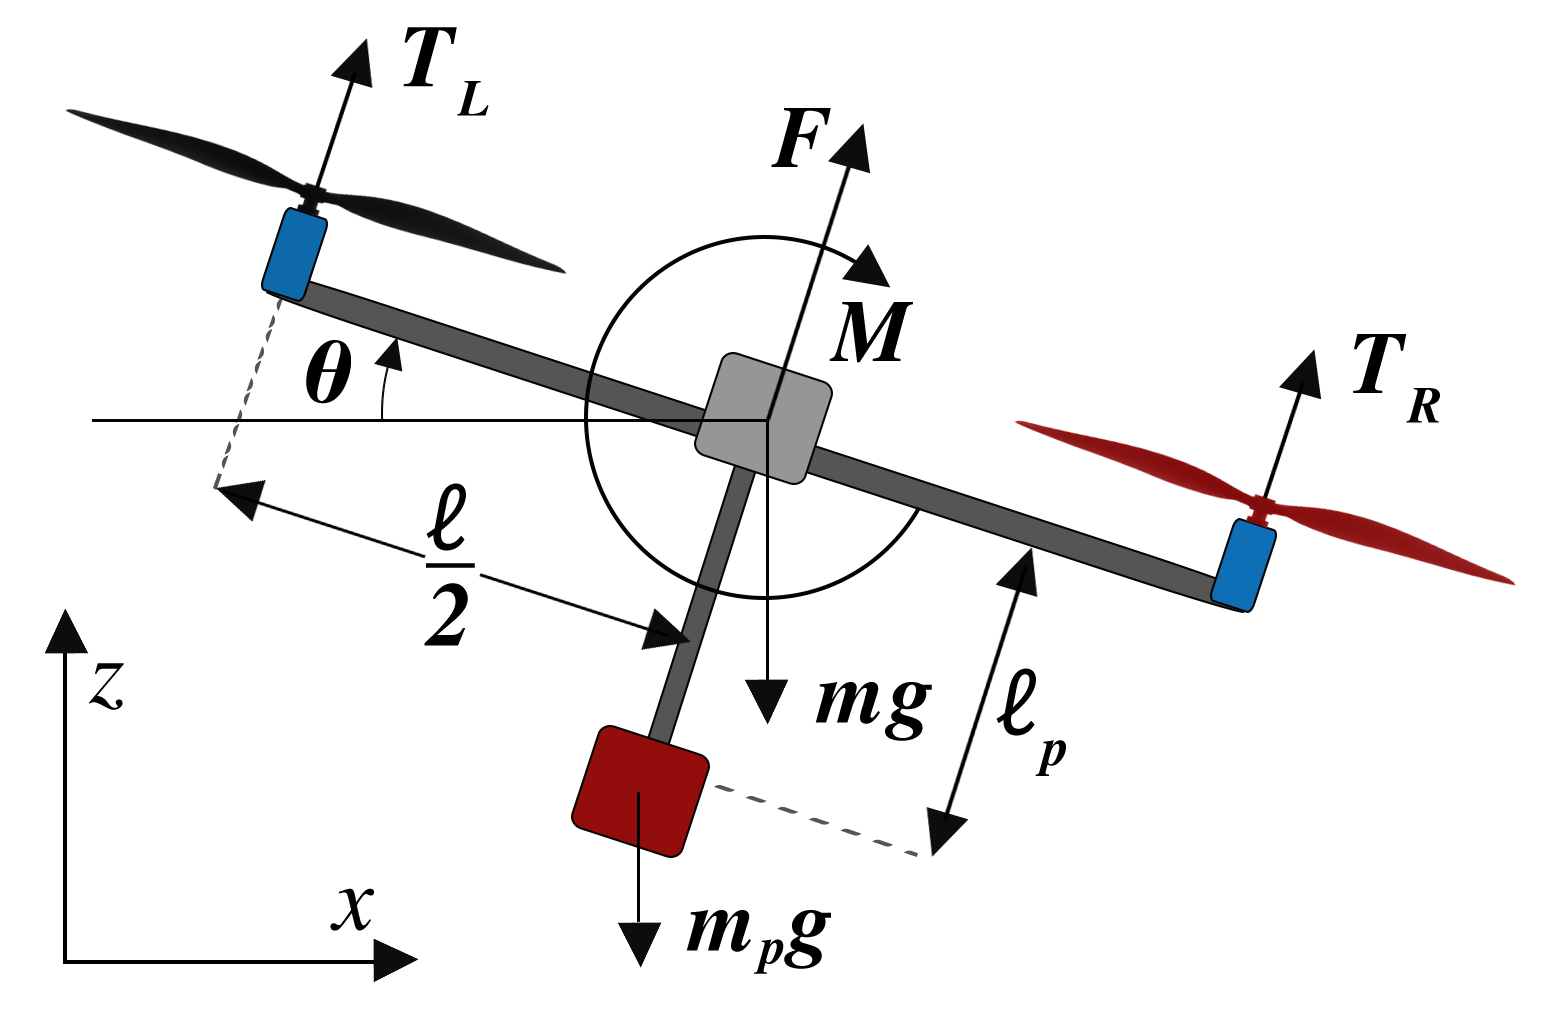
\includegraphics[width=0.42\textwidth]{tandem_rotor}
	\caption{Diagram of simplified planar quadrotor (tandem-rotor) constrained to $xz$-plane}
\end{figure}

For motion-planning purposes, this system can be linearized about hover ($\theta = 0, F_0 = (m+m_p)g$), and simplified by assuming negligible air drag and no external disturbances
\begin{equation}
	\dot X = \begin{bmatrix}
		\mathbf{0}_3 & \mathbf{I}_3 \qquad \\ \footnotesize
		\begin{bmatrix} 0 & 0 & -g \\
		0 & 0 & 0 \\
		0 & 0 & \frac{m_p \ell_p g}{I_{yy}} \end{bmatrix}\normalsize & \mathbf{0}_3 \qquad
	\end{bmatrix} X + \begin{bmatrix}
		\mathbf{0}_2 \\ \mathbf{0}_2 \\
		\footnotesize \begin{bmatrix}\frac{1}{m+m_p} & 0 \\ 0 & \frac{1}{I_{yy}} \end{bmatrix} \normalsize
	\end{bmatrix} \begin{bmatrix}
		\Delta F_T \\ M_T
	\end{bmatrix}
\end{equation}
%\begin{multline}
%	\dot X = \begin{bmatrix}
%		0 & 0 & 0 & 1 & 0 & 0 \\
%		0 & 0 & 0 & 0 & 1 & 0 \\
%		0 & 0 & 0 & 0 & 0 & 1 \\
%		0 & 0 & -g & 0 & 0 & 0 \\
%		0 & 0 & 0 & 0 & 0 & 0 \\
%		0 & 0 & m_p \ell_p g / I_{yy} & 0 & 0 & 0 \\		
%	\end{bmatrix} \begin{bmatrix}
%		x \\ z \\ \theta \\ \dot x \\ \dot z \\ \dot \theta
%	\end{bmatrix}  \\ + \begin{bmatrix}
%		0 & 0 \\ 0 & 0 \\ 0 & 0 \\ 0 & 0 \\
%		\frac{1}{m+m_p} & 0 \\ 0 & \frac{1}{I_{yy}}
%	\end{bmatrix} \begin{bmatrix}
%		\Delta F_T \\ M_T
%	\end{bmatrix}
%	\label{nonlin_dynamics}
%\end{multline}
\noindent where $\Delta F_T$ is deviation from $F_0$, the thrust required for hover. \begin{comment}
%\begin{equation}
%	\dot X = \begin{bmatrix}
%		\mathbf{0}_3 & \mathbf{I}_3 \qquad \\ \footnotesize
%		\begin{bmatrix} 0 & 0 & -g \\
%		0 & 0 & 0 \\
%		0 & 0 & m_p \ell_p g / I_{yy} \end{bmatrix}\normalsize & \mathbf{0}_3 \qquad
%	\end{bmatrix} \begin{bmatrix}
%		x \\ z \\ \theta \\ \dot x \\ \dot z \\ \dot \theta
%	\end{bmatrix} + \begin{bmatrix}
%		0 & 0 \\ 0 & 0 \\ 0 & 0 \\ 0 & 0 \\
%		\frac{1}{m+m_p} & 0 \\ 0 & \frac{1}{I_{yy}}
%	\end{bmatrix} \begin{bmatrix}
%		\Delta F_T \\ M_T
%	\end{bmatrix}
%\end{equation}

%
%With different input definition:
%\begin{equation*}
%	\dot X = \underbrace{\begin{bmatrix}
%		\dot x \\ \dot z \\ \dot \theta \\ 0 \\ -g \\ \frac{m_p \ell_p g \sin(\theta)}{I_{yy}}
%	\end{bmatrix}}_{f(X,t)} + \underbrace{\begin{bmatrix}
%		0 & 0 \\ 0 & 0 \\ 0 & 0 \\ \frac{-\sin(\theta)}{m+m_p} & \frac{-\sin(\theta)}{m+m_p} \\
%		\frac{\cos(\theta)}{m+m_p} & \frac{\cos(\theta)}{m+m_p} \\ \frac{\ell}{2I_{yy}} & \frac{-\ell}{2I_{yy}}
%	\end{bmatrix}}_{G(X,t)} \underbrace{\begin{bmatrix}
%		T_L \\ T_R
%	\end{bmatrix}}_{u(t)}
%\end{equation*}
%
%\begin{equation*}
%	\begin{bmatrix}
%		\ddot x \\ \ddot z \\ \ddot \theta
%	\end{bmatrix} = \begin{bmatrix}
%		0 \\ -g \\ \frac{m_p \ell_p g \sin(\theta)}{I_{yy}}
%	\end{bmatrix} + \begin{bmatrix}
%		\frac{-\sin(\theta)}{m+m_p} & \frac{-\sin(\theta)}{m+m_p} \\
%		\frac{\cos(\theta)}{m+m_p} & \frac{\cos(\theta)}{m+m_p} \\ \frac{\ell}{2I_{yy}} & \frac{-\ell}{2I_{yy}}
%	\end{bmatrix} \begin{bmatrix}
%		T_L \\ T_R
%	\end{bmatrix}
%\end{equation*}

Further, the vehicle state can be augmented to include first-order actuator dynamics
\small
\begin{multline*}
	\begin{bmatrix}
		\dot x \\ \dot z \\ \dot \theta \\ \ddot x \\ \ddot z \\ \ddot \theta \\ \dot \Omega_L \\ \dot \Omega_R
	\end{bmatrix} = \begin{bmatrix} 0 \\ 0 \\ 0 \\
		\frac{-\bar{c}_d |\dot x|\dot x}{m+m_p} - \frac{c_t \sin(\theta)}{m+m_p} (\Omega_L^2 + \Omega_R^2) \\ 
		\frac{-\bar{c}_d |\dot z|\dot z}{m+m_p} - g + \frac{c_t \cos(\theta)}{m+m_p}(\Omega_L^2 + \Omega_R^2) \\ 
		\frac{m_p \ell_p g \sin(\theta)}{I_{yy}} + \frac{\ell c_t}{2I_{yy}}(\Omega_L^2 - \Omega_R^2) \\
		-\frac{\Omega_L}{\tau} \\ -\frac{\Omega_R}{\tau}
	\end{bmatrix}  \\ + \begin{bmatrix}
		0 & 0 \\ 0 & 0 \\ 0 & 0 \\ 0 & 0 \\ 0 & 0 \\ 0 & 0 \\ 1/\tau & 0 \\ 0 & 1/\tau
	\end{bmatrix} \begin{bmatrix}
		u_L \\ u_R
	\end{bmatrix}
\end{multline*} \normalsize
\noindent where $\Omega_L$ and $\Omega_R$ are the angular velocities of the left and right rotors, respectively, and $c_t$ is a coefficient of thrust.
\end{comment} 
The dynamics of Equation \ref{nonlin_dynamics} are used for control purposes in this paper, and the controller is designed for robustness to both unmodeled actuator dynamics and external disturbances (wind).

\subsection{Nested Control Formulation}
The system is underactuated and non-holonomic, as there are two actuators and three degrees of freedom, so we cannot drive the states $(x, z, \theta)$ to any desired configuration simultaneously. Instead, a nested (hierarchical) controller must be designed, and the following subset of the dynamics is chosen as the outer loop
\begin{equation}
	\begin{bmatrix}
		\dot x \\ \dot z \\ \ddot x \\ \ddot z
	\end{bmatrix} = \begin{bmatrix}
		\dot x \\ \dot z \\ \frac{-\bar{c}_d |\dot x|\dot x}{m+m_p} + \frac{F \sin(\theta)}{m+m_p} \\ \frac{-\bar{c}_d |\dot z|\dot z}{m+m_p} + \frac{F \cos(\theta)}{m+m_p} - g
	\end{bmatrix}
\end{equation}
\noindent where these dynamics will be used to define $F_{T,d} = T_{L,d} + T_{R,d}$, and $\theta$ is fed to the inner loop as $\theta_d$. The inner loop dynamics is then
\begin{equation}
	\begin{bmatrix}
		\dot \theta \\ \ddot \theta 
	\end{bmatrix} = \begin{bmatrix}
		\dot \theta \\ \frac{m_p \ell_p g \sin(\theta) + M}{I_{yy}}
	\end{bmatrix}
\end{equation}
\noindent where the control law will be defined to give $M_{T,d} = (T_{L,d} - T_{R,d})\ell/2$.

\subsection{Actuator Dynamics}
Desired control inputs $F_{T,d} = (T_{L,d} + T_{R,d})$, and $M_{T,d} = (T_{L,d} - T_{R,d})\ell/2$ are mapped to the actuators as
\begin{align*}
	T_L &= T_{L,d} \frac{c_t}{\tau s + 1} = (F_{T,d}/2 + M_{T,d} / \ell) \frac{c_t}{\tau s + 1}\\
	T_R &= T_{R,d} \frac{c_t}{\tau s + 1} = (F_{T,d}/2 - M_{T,d} / \ell) \frac{c_t}{\tau s + 1}
\end{align*}
\noindent where $c_t$ is a coefficient of thrust, $\tau$ is a time constant of the unmodeled first-order actuator dynamics, and $T_L$ and $T_R$ are constrained to the interval $\begin{bmatrix}0, & T_{max}\end{bmatrix}$.

\subsection{External Disturbances}
The control law is designed to be robust to external disturbances, representing wind. Wind is modeled as an addition to the force and moment dynamics of the vehicle so that
\begin{align}
	F &= F_T + F_W \\
	M &= M_T + M_W
\end{align}
where the forces and moments are filtered white noise defined as
\begin{align}
	F_W(s) &= \nu(t) \sum_{i=1}^N \frac{k_{F,i}}{a_{2,i}s^2 + a_{1,i}s + 1} 	\label{wind_eqn1} \\
	M_W(s) &= \nu(t) \sum_{i=1}^N \frac{k_{M,i}}{b_{2,i}s^2 + b_{1,i}s + 1} \label{wind_eqn2}
\end{align}
and $\nu \sim \mathcal{N}(0,\sigma^2)$.

%It is worth noting that the system has the property of differential flatness (all state variables and inputs can be expressed as smooth functions of flat outputs $[x, z]$ and derivatives).

\section{Optimal Kinodynamic Motion Planning}
For a linear system without state constraints or input constraints, an optimal trajectory between states $\mathbf{x}_0$ and $\mathbf{x}_1$ is straightforward to find. If we wish to minimize a cost which weighs arrival time and control effort (or deviation from a control set-point), this problem can be formulated as follows (adapted from \cite{webb2013kinodynamic}). Consider a plant with dynamics
\begin{equation}
	\dot{\mathbf{x}} (t) = A \mathbf{x}(t) + B \mathbf{u}(t) + \mathbf{c}	
\end{equation}

A trajectory is defined as $\pi = (\mathbf{x}(), \mathbf{u}(), \tau)$ for $t = 0\ldots \tau$, $\mathbf{x}(0) = \mathbf{x}_0$, $\mathbf{x}(\tau) = \mathbf{x}_1$. We can define the cost of this trajectory as
\begin{equation}
	c(\pi) = \int_0^\tau (1 + \mathbf{u}(t)^T R \mathbf{u}(t))dt
\end{equation}
where $R$ is a problem-dependent control effort weighting matrix. The goal is then to find the optimal trajectory $\pi^*(\mathbf{x}_0, \mathbf{x}_1) = (\mathbf{x}(), \mathbf{u}(), \tau^*)$ which minimizes $c$. Before finding the optimal state and input trajectory, the optimal arrival time $\tau^* = \text{argmin}\{ c(\tau) \}$ can be determined. The derivative of the optimal trajectory cost is given by
\begin{equation}
	\dot{c}(\tau) = 1 - 2(A \mathbf{x}_1 + c)^T \mathbf{d}(\tau) - \mathbf{d}(\tau)^T B R^{-1} B^T \mathbf{d}(\tau)
\end{equation}
and 
\begin{equation}
	\mathbf{d}(\tau) = G(\tau)^{-1} (\mathbf{x}_1 - \bar{\mathbf{x}}(\tau))
\end{equation}
where $G(\tau)$ is weighted controllability Gramian and $\bar{\mathbf{x}}(\tau)$  is zero-input state solution with $\bar{\mathbf{x}}(0) = \mathbf{x}_0$. $G(t)$ has dynamics
\begin{equation}
	\dot{G}(t) = A G(t) + G(t) A^T + B R^{-1} B^T, \qquad G(0) = \mathbf{0}
\end{equation}

Unless $A$ is nilpotent ($A^n = 0$ where $A \in \mathbb{R}^{n \times n}$), $\tau^*$ must be solved for numerically. To compute the optimal trajectory $\pi^*(\mathbf{x}_0, \mathbf{x}_1) = (\mathbf{x}(), \mathbf{u}(), \tau^*)$, the following composite differential equation is constructed
\begin{equation}
	\begin{bmatrix}
		\dot{\mathbf{x}}(t) \\ \dot{\mathbf{y}}(t)
	\end{bmatrix} = \begin{bmatrix}
		A & B R^{-1} B^T \\ 0 & -A^T
	\end{bmatrix} \begin{bmatrix}
		\mathbf{x}(t) \\ \mathbf{y}(t)
	\end{bmatrix} + \begin{bmatrix}
		\mathbf{c} \\ \mathbf{0}
	\end{bmatrix}
\end{equation}
with final condition
\begin{equation}
	\begin{bmatrix}
		\mathbf{x}(\tau^*) \\ \mathbf{y}(\tau^*)
	\end{bmatrix} = \begin{bmatrix}
		\mathbf{x}_1 \\ \mathbf{d}(\tau^*)
	\end{bmatrix}
\end{equation}

This can be integrated backwards in time (numerically) to find the optimal trajectory. If the optimal trajectory is infeasible (state or input constraints not satisfied, or obstacles encountered), points are sampled randomly from the state space to provide intermediate connections between the start and goal states until a feasible plan is found. The details of this algorithm are not covered here, but details can be found in \cite{webb2013kinodynamic}.

\section{Robust Adaptive Sliding Control}
\begin{figure}
	\centering
	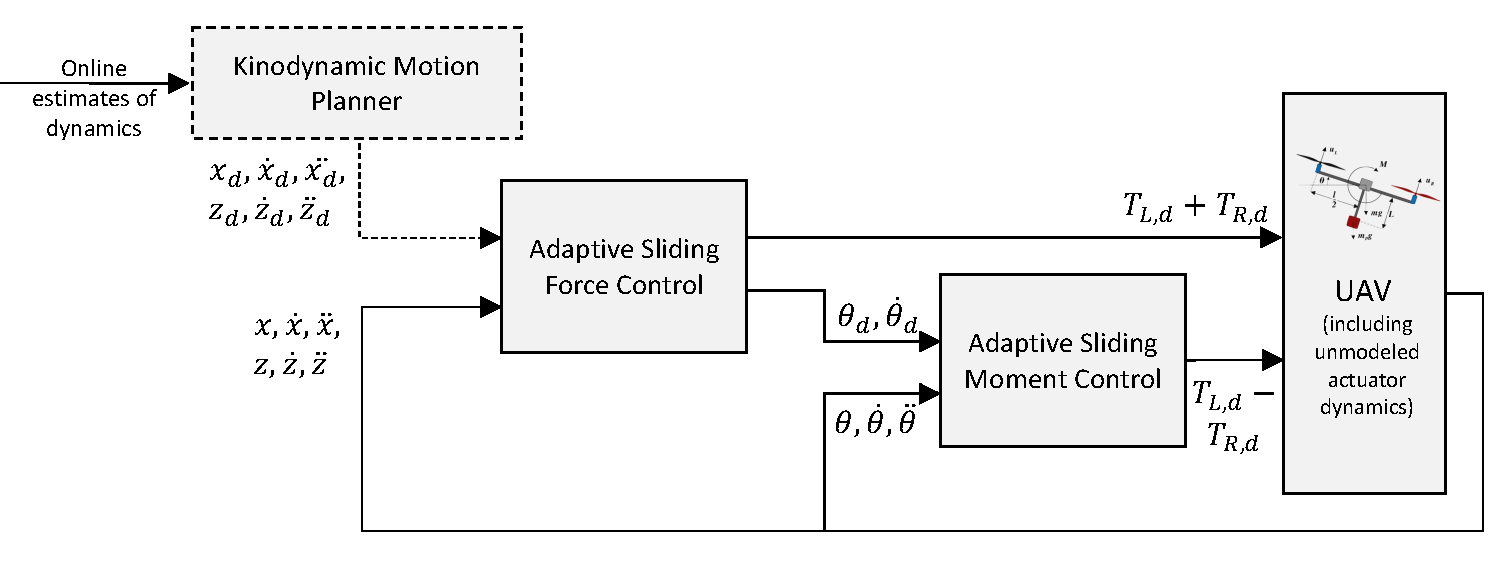
\includegraphics[width=0.5\textwidth]{block_diagram}
	\caption{High-level block diagram of control structure}
	\label{block}
\end{figure}

\subsection{Closed-Loop Adaptive Trajectory Control}
The position dynamics of the tandem-rotor vehicle, as introduced above, are given by
\begin{align}
	(m+m_p) \ddot x + \bar{c}_d |\dot x| \dot x &= (F_T + F_W) \sin(\theta) \\
	(m+m_p) (\ddot z + g) + \bar{c}_d |\dot z| \dot z &= (F_T + F_W) \cos(\theta)
\end{align}
As shown in Figure \ref{block}, the outer loop controller takes a desired trajectory from motion planner ($x_d(t), \dot x_d(t), \ddot x_d(t), z_d(t), \dot z_d(t), \ddot z_d(t)$), which is dynamically feasible to the extent that the motion planner knows the dynamics of the vehicle, and excluding external disturbances. We define sliding variables
\begin{align}
	s_z &= \dot{\tilde{z}} + \lambda \tilde z \\
	s_x &= \dot{\tilde{x}} + \lambda \tilde x
\end{align}
where $\tilde{z} = z(t) - z_d(t)$, $\tilde{x} = x(t) - x_d(t)$. The reference signals $\ddot{z}_r = \ddot{z}_d - \lambda \dot{\tilde{z}}$ and $\ddot{x}_r = \ddot{x}_d - \lambda \dot{\tilde{x}}$ are defined for notational simplicity. The outer loop control law is then defined as
\begin{equation}
	\underbrace{\begin{bmatrix}
		u_1 \\ u_2
	\end{bmatrix}}_{u_{out}} = \underbrace{\begin{bmatrix}
		\ddot{z}_r + g, & |\dot z|\dot z \\ \ddot{x}_r, & |\dot x|\dot x 
	\end{bmatrix}}_{Y_{out}} \underbrace{\begin{bmatrix}
		\hat{a}_{out,1} \\
		\hat{a}_{out,2}
	\end{bmatrix}}_{\hat{a}_{out}} - \begin{bmatrix}
		k_z \text{sat}(\frac{s_z}{\Phi_z}) \\ k_x \text{sat}(\frac{s_x}{\Phi_x})
	\end{bmatrix} 
\end{equation}

The true parameter vector 
\begin{equation}
	a_{out} = \begin{bmatrix}
		 \frac{m+m_p}{c_t}\\
		 \frac{\bar{c}_d}{c_t}
	\end{bmatrix}
\end{equation} is replaced by the online estimate $\hat{a}_{out}$ with the adaptive control law
\begin{equation}
	\dot{\hat{a}}_{out} = - \gamma Y^T_{out} \begin{bmatrix}
		s_{\Delta z} \\ s_{\Delta x}
	\end{bmatrix}
\end{equation}
which makes use of
\begin{align}
	s_{\Delta z} = s_z - \Phi_z \text{sat}(\frac{s_z}{\Phi_z})\\
	s_{\Delta x} = s_x - \Phi_x \text{sat}(\frac{s_x}{\Phi_x})
\end{align}
to create a dead-zone in which adaptation is suspended \cite{slotine1991applied}. The desired control signals are computed using nonlinear transformations
\begin{align}
	\theta_d &= -\tan^{-1}{(\frac{u_2}{u_1})} \\
	F_{T,d} &= \sqrt{u_1^2 + u_2^2}
\end{align}

\subsection{Adaptive Pitch Angle Control}
The inner loop controller tracks the desired pitch angle, which allows the vehicle thrust to be oriented in the correct direction. As shown in Section II, the vehicle's rotational dynamics are given by
\begin{equation}
	I_{yy} \ddot{\theta} - m_p \ell_p g \sin(\theta) = M_T + M_W
\end{equation}
where the nonlinearity in these dynamics arises from the payload of unknown mass and moment from the vehicle center of mass. Similar to the outer loop controller in the section above, we define a sliding variable
\begin{equation}
	s_\theta = \dot{\tilde{\theta}} + \lambda \tilde \theta
\end{equation}
where $\tilde{\theta} = \theta(t) - \theta_d(t)$, as well as reference angular acceleration $\ddot{\theta}_r = \ddot{\theta}_d - \lambda \dot{\tilde{\theta}}$. Inner loop pitch angle control using $\theta_d = -\tan^{-1}{(\frac{u_2}{u_1})}$ gives control law
\begin{equation}
	M_{T,d} = u_3 = \underbrace{\begin{bmatrix}
		\ddot{\theta}_r & \sin{(\theta)}
	\end{bmatrix}}_{Y_{in}} \underbrace{\begin{bmatrix}
		\hat{a}_{in,1} \\
		\hat{a}_{in,2}
	\end{bmatrix}}_{\hat{a}_{in}} - k_\theta \text{sat}(\frac{s_\theta}{\Phi_\theta})
\end{equation}

The true parameter vector
\begin{equation}
	a_{in} = \begin{bmatrix}
			\frac{I_{yy}}{c_t} \\
			\frac{-m_p \ell_p}{c_t}
		\end{bmatrix}
\end{equation}
is estimated by $\hat{a}_{in}$ and adaptive control law
\begin{equation}
	\dot{\hat{a}}_{in} = - \Gamma Y^T_{in} s_{\Delta \theta}
\end{equation}
with 
\begin{equation}
	s_{\Delta\theta} = s_{\theta} - \Phi_{\theta} \text{sat}(\frac{s_{\theta}}{\Phi_{\theta}})
\end{equation}

As stated above, the commands sent to the vehicle's motors are then
\begin{align}
	T_{L,d} = \frac{F_{T,d}}{2} + \frac{M_{T,d}}{\ell}\\
	T_{R,d} = \frac{F_{T,d}}{2} - \frac{M_{T,d}}{\ell}
\end{align}

\section{Controller Stability}
\subsection{Inner Loop}
Convergence of the inner loop controller to desired pitch angle can be shown for the controller above in the presence of external disturbances. Define Lyapunov function candidate
\begin{equation}
	V = \frac{1}{2}s_{\Delta \theta} I_{yy} s_{\Delta \theta} + \frac{1}{2}\tilde{a}_{in}^T \Gamma^{-1} \tilde{a}_{in}
\end{equation} 
and differentiate, to get
\begin{align*}
	\dot V &= I_{yy} s_{\Delta \theta} \dot s + \dot{\hat{a}}_{in} \Gamma^{-1} \tilde{a}_{in} \\
	~ &= s_{\Delta \theta} (I_{yy}\ddot{\theta} - I_{yy}\ddot{\theta}_r) + \dot{\hat{a}}_{in} \Gamma^{-1} \tilde{a}_{in} \\
	~ &= s_{\Delta \theta} (u - Y_{in}a_{in} + M_W) + \dot{\hat{a}}_{in} \Gamma^{-1} \tilde{a}_{in} \\
	~ &= - s_{\Delta \theta} k_\theta \text{sat}\left(\frac{s_\theta}{\Phi_\theta}\right) + s_{\Delta \theta}(Y_{in} \tilde{a}_{in} + M_W) \\ ~& \qquad ~\qquad ~ \qquad~ \qquad ~\qquad + \dot{\hat{a}}_{in} \Gamma^{-1} \tilde{a}_{in}
\end{align*}

Substituting in the adaptation law, 
\begin{equation}
	\dot V = - k_\theta |s_{\Delta \theta}| + s_{\Delta \theta} M_W
\end{equation}

For a negative semi-definite $\dot V$, it is necessary to choose $k_\theta = |M_{W,max}| + \eta$, $\eta > 0$ so that $\dot{V} \leq -\eta |s_{\Delta \theta}|$. Then by Barbalat's Lemma, $\dot{V} \rightarrow 0$ as $t \rightarrow \infty$, implying $s_{\Delta \theta} \rightarrow 0$ and $\theta \rightarrow \theta_d$. 

When actuators have dynamics which are unaccounted for in the control law, it is necessary to choose $\lambda_{il}$ (subscript for ``inner loop'') for the sliding controller so that the bandwidth of the controller does not exceed that of the actuators. According to the design guidelines given in \cite{slotine1991applied}, it is desirable that $\lambda_{il} \leq \frac{1}{3 \tau}$, where $\tau$ is the actuator time constant (given in \cite{slotine1991applied} for time delay, but applied here for first order dynamics).

\subsection{Outer Loop}
Stability of the outer loop controller can be established in a manner similar to that of the inner loop. The inner loop dynamics, which is stable when the controller bandwidth is sufficiently low compared to that of the actuators, can then be considered slower actuator dynamics with break frequency $\lambda_{il}$. This implies that the bandwidth of the outer loop will need to be low compared to that of the inner loop ($\lambda_{ol} < \lambda_{il} < \lambda_{act}$). This is the design principle used in the following numerical example, where the controller is demonstrated in simulation. 

To show stability, we first define 
\begin{align*}
	\mathbf{s}_\Delta &= \begin{bmatrix}
	s_{\Delta x}, & s_{\Delta z}
\end{bmatrix}^T \\
	\mathbf{k} &= \text{diag}\begin{bmatrix}
	k_x, & k_z
\end{bmatrix} \\
	\mathbf{F}_W &= \begin{bmatrix}
	F_W \sin(\theta), & F_W \cos(\theta)\end{bmatrix}^T \\
	u &= \begin{bmatrix}
		u_1, & u_2
	\end{bmatrix}^T
\end{align*}
and then proceed to define Lypaunov function candidate
\begin{equation}
	V = \frac{1}{2}\mathbf{s}_{\Delta}^T (m+m_p) \mathbf{s}_{\Delta} + \frac{1}{2}\tilde{a}_{out}^T \Gamma^{-1} \tilde{a}_{out}
\end{equation}
and differentiate, which gives
\begin{align*}
	\dot V &= (m+m_p) \mathbf{s}_\Delta^T \dot{\mathbf{s}} + \dot{\hat{a}}_{out}^T \Gamma^{-1} \tilde{a}_{out} \\
	~ &= \mathbf{s}_\Delta^T (u - Y_{out} a_{out} + \mathbf{F}_W)  + \dot{\hat{a}}_{out}^T \Gamma^{-1} \tilde{a}_{out} \\
	~ &= -\mathbf{s}_\Delta^T \mathbf{k} \text{sat}\left(\frac{\mathbf{s}}{\Phi}\right) + \mathbf{s}_\Delta^T(Y_{out} \tilde{a}_{out} + \mathbf{F}_W) \\
	~ & \qquad ~\qquad ~ \qquad~ \qquad ~\qquad + \dot{\hat{a}}_{out}^T \Gamma^{-1} \tilde{a}_{out}\\
\end{align*}
leading as before to 
\begin{equation}
	\dot{V} = -\mathbf{s}_\Delta^T \mathbf{k} \text{sat}\left(\frac{\mathbf{s}}{\Phi}\right) + \mathbf{s}_\Delta^T \mathbf{F}_W
\end{equation}

As in the inner loop system, we must then choose $k_x$ and $k_z$ such that $|\mathbf{k}| = |\mathbf{F}_W| + \eta, \eta > 0$, so that $\dot{V} \leq -\eta |s_{\Delta}|$. Then by Barbalat's Lemma, $\dot{V} \rightarrow 0$ as $t \rightarrow \infty$, implying $\mathbf{s}_{\Delta} \rightarrow 0$ and $(x,\quad z) \rightarrow (x_d,\quad z_d)$. 

\section{Numerical Simulation}
\begin{figure}
	\centering
	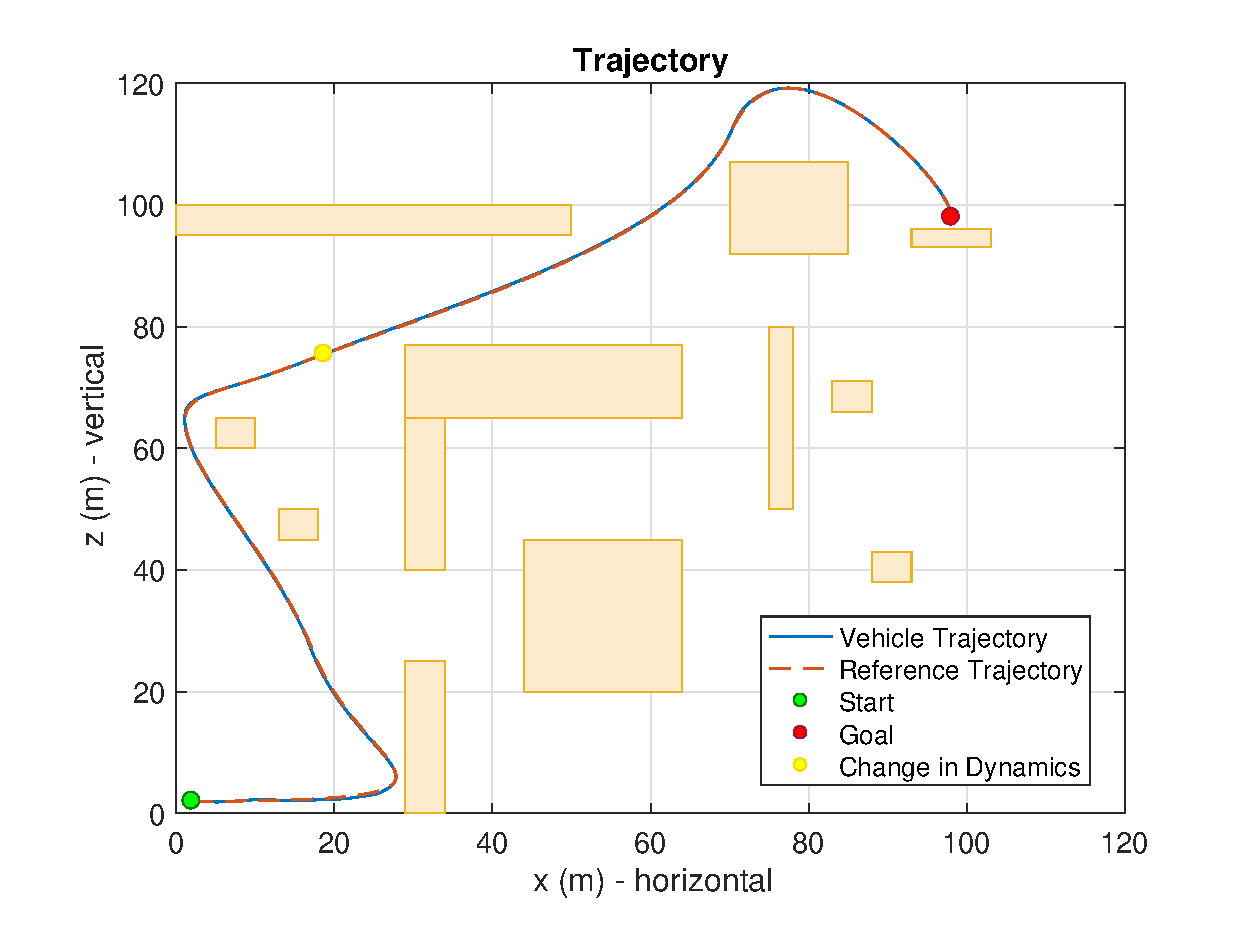
\includegraphics[width=0.5\textwidth]{traj2}
	\caption{Tandem-rotor vehicle trajectory}
	\label{traj1}
\end{figure}
\begin{figure}[thbp!]
	\centering
	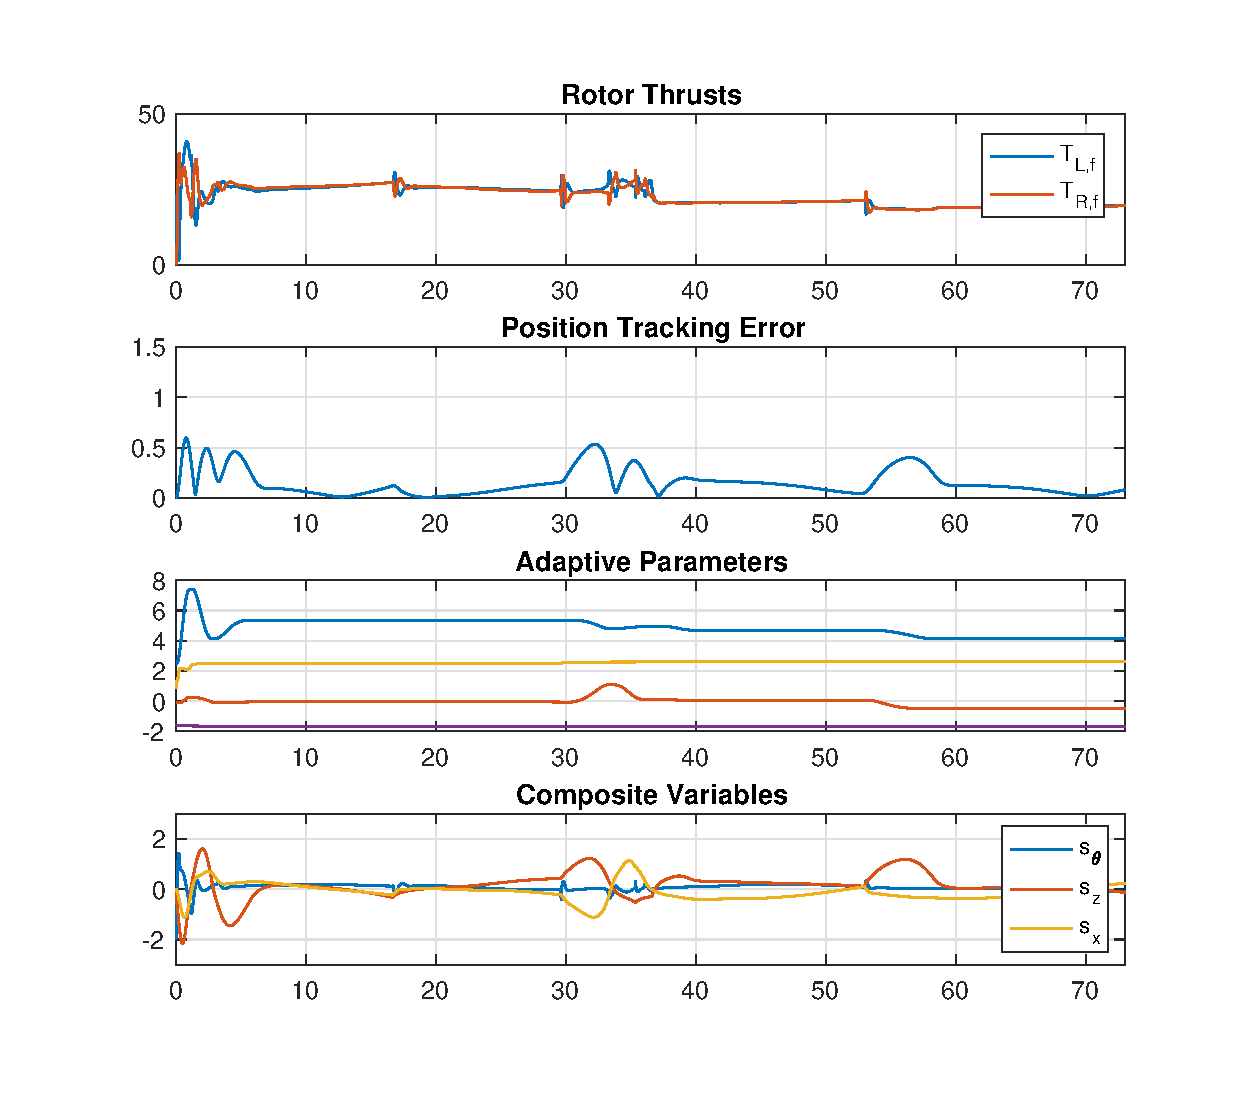
\includegraphics[width=0.5\textwidth]{data3}
	\caption{Data associated with trajectory in Fig. \ref{traj1}}
	\label{data1}
\end{figure}
 
The numerical simulation in Figures \ref{traj1} and \ref{data1} uses the parameters given in Tables \ref{plant_params} and \ref{ctrl_params}. Initial estimates $\hat{a}_{out}$ and $\hat{a}_{in}$ are initialized as $0.5 a_{out}$ and $0.5 a_{in}$ respectively. As shown in Table \ref{plant_params}, the values of $m_p$, $\ell_p$, and $c_t$ change during the simulation, and the controller adapts.

Wind is modeled as an external disturbance, as given in Equations \ref{wind_eqn1} and \ref{wind_eqn2}, given numerically by \small
\begin{align}
	F_W(s) &= \nu(t) \left[ \frac{15}{6s^2 + 5s + 1} - \frac{40}{16s^2 + 8s + 1} \right] \\
	M_W(s) &= \nu(t) \frac{2}{4s^2 + 4s + 1}
\end{align} \normalsize
where $\nu(t) \sim \mathcal{N}(0,1)$. From this simulation (and the simulations in the Appendix used for validation and tuning), it is clear that the controller achieves the design goals. Namely, the controller adapts online to the unknown parameters, while remaining robust to external disturbances, unmodeled actuator dynamics, and the separation of translational and rotational vehicle dynamics. Comparisons to other controllers, and details of tuning can be found in the Appendix of this paper.

\begin{table}[h!]
	\renewcommand{\arraystretch}{1.2}
	\centering
    \begin{tabular}{|lll|} \hline
    ~ & $t < 36$ s & $t \geq 36$ s \\ \hline
    $\ell$ (m) & 0.5 & - \\
    $\ell_p$ (m) & 0.4 & 0.3 \\
    $m$ (kg) & 3.0 & - \\
    $m_p$ (kg) & 2.0 & 1.0 \\
    $I_{yy}$ (kg$\cdot$m$^2$) & 0.414 & 0.184 \\ 
    $c_t$ (s) & 1.0 & 0.92 \\
    $\bar{c}_d$ (s) & 1.57 & - \\
    $\tau$ (s) & 0.05 & - \\
    $T_{max}$ (N) & 80 & - \\ \hline
    \end{tabular}
    \caption{Vehicle parameters, which change during simulation}
    \label{plant_params}
\end{table}
\begin{table}[h!]
	\renewcommand{\arraystretch}{1.2}
	\centering
    \begin{tabular}{|llll|} \hline
    Parameter & $(\cdot)_x$ & $(\cdot)_z$ & $(\cdot)_\theta$ \\ \hline
    $\Phi$ & 0.4 & 0.4 & 0.1 \\    
    $\lambda$ & 2.0 & 2.0 & 6.0 \\
    $k$ & 3.0 & 3.0 & 0.05 \\
    $\gamma$ & 1.0 & 1.0 & 1.0 \\ \hline
    \end{tabular}
    \caption{Controller parameters}
    \label{ctrl_params}
\end{table}

\section{Conclusions and Future Work}
In this paper, a controller was designed and evaluated in a simulation environment for a planar quadrotor (tandem-rotor) vehicle, which is carrying a payload modeled as a point-mass of unknown mass and distance from the vehicle's center of mass. A nested control formulation is used, with an outer loop translational controller and an inner loop rotational controller, which together adapt to changes in payload, actuator, and damping parameters $(m_p, \ell_p, c_t, \bar{c}_d$). The controller demonstrates its ability to track the reference trajectory even in the presence of unmodeled actuator dynamics, external disturbances, and adaptation in two hierarchical control loops.

There are many possible extensions for the work done in this paper. The work can be extended to the full 6DOF vehicle, which can move in 3D space. This takes the state-space from 6-dimensional to 12-dimensional. The actuator dynamics could be included in the controller design. An adaptive controller could be designed to counteract the effects of unknown and slowly time-varying winds, by estimating the magnitude and direction of wind online. Another problem could consider a payload whose mass is not coincident with the plane of symmetry of the vehicle. If persistency of excitation can be guaranteed online, then estimates of the unknown parameters, $m_p$ and $\ell_p$ can be used for online replanning with the kinodynamic motion planner whenever these parameters change.


\nocite{slotine1991applied, karaman2010optimal, webb2013kinodynamic, allen2015toward, bouabdallah2007full}
\bibliographystyle{ieeetr}
\bibliography{2152_bib}

\newpage
\appendix
Here, the final controller (presented in section above) is compared to several variants. In all these examples there are unmodeled actuator dynamics and external disturbances, as described above. The reference trajectory in all these examples is defined as
\begin{equation}
	\underbrace{\begin{bmatrix}
		x_d \\ \dot{x}_d \\ \ddot{x}_d \\ z_d \\ \dot{z}_d \\ \ddot{z}_d
	\end{bmatrix}}_{X_d} = \begin{bmatrix}
		10 \cos(\frac{2 \pi t}{T_1}) + 0.2 \cos(\frac{2 \pi t}{T_2}) \\
		-20 \frac{\pi}{T_1} \sin(\frac{2 \pi t}{T_1}) - 0.4 \frac{\pi}{T_2} \sin(\frac{2 \pi t}{T_2}) \\
		-40 (\frac{\pi}{T_1})^2 \cos(\frac{2 \pi t}{T_1}) - 0.8 (\frac{\pi}{T_2})^2 \cos(\frac{2 \pi t}{T_2}) \\
		10 \sin(\frac{2 \pi t}{T_1}) + 0.2 \cos(\frac{2 \pi t}{T_2}) \\
		20 \frac{\pi}{T_1} \cos(\frac{2 \pi t}{T_1}) - 0.4 \frac{\pi}{T_2} \sin(\frac{2 \pi t}{T_2}) \\
		-40 (\frac{\pi}{T_1})^2 \sin(\frac{2 \pi t}{T_1}) - 0.8 (\frac{\pi}{T_2})^2 \cos(\frac{2 \pi t}{T_2})
	\end{bmatrix}
\end{equation} with $T_1 = 20s$ and $T_2 = 5s$.

\begin{table}[h!]
	\renewcommand{\arraystretch}{1.2}
	\centering
    \begin{tabular}{|lll|} \hline
    ~ & $t < 150$ s & $t \geq 150$ s \\ \hline
    $\ell$ (m) & 0.5 & - \\
    $\ell_p$ (m) & 0.4 & 0.3 \\
    $m$ (kg) & 3.0 & - \\
    $m_p$ (kg) & 2.0 & 1.0 \\
    $I_{yy}$ (kg$\cdot$m$^2$) & 0.414 & 0.184 \\ 
    $c_t$ (s) & 1.0 & 0.92 \\
    $\bar{c}_d$ (s) & 1.57 & - \\
    $\tau$ (s) & 0.05 & - \\
    $T_{max}$ (N) & 80 & - \\ \hline
    \end{tabular}
    \caption{Vehicle parameters, which change during simulation}
    \label{plant_params_appendix}
\end{table}

\subsection{Full (Final) Controller}
The test of this controller is shown in Figures \ref{circle_traj_1} and \ref{circle_data_1}. In this example, tracking performance is good over the entire simulation, including the initial phase where adaptive parameters are initialized to $50\%$ of their true values, as well as the phase following a change in plant parameters ($m_p, \ell_p, c_t$) at $t = 150s$.

\begin{table}[h!]
	\renewcommand{\arraystretch}{1.2}
	\centering
    \begin{tabular}{|llll|} \hline
    Parameter & $(\cdot)_x$ & $(\cdot)_z$ & $(\cdot)_\theta$ \\ \hline
    $\Phi$ & 0.4 & 0.4 & 0.1 \\    
    $\lambda$ & 2.0 & 2.0 & 6.0 \\
    $k$ & 6.0 & 6.0 & 0.05 \\
    $\gamma$ & 0.2 & 0.2 & 2.0 \\ \hline
    \end{tabular}
    \caption{Controller parameters}
    \label{ctrl_params_appendix}
\end{table}

\begin{figure}[h!]
	\centering
	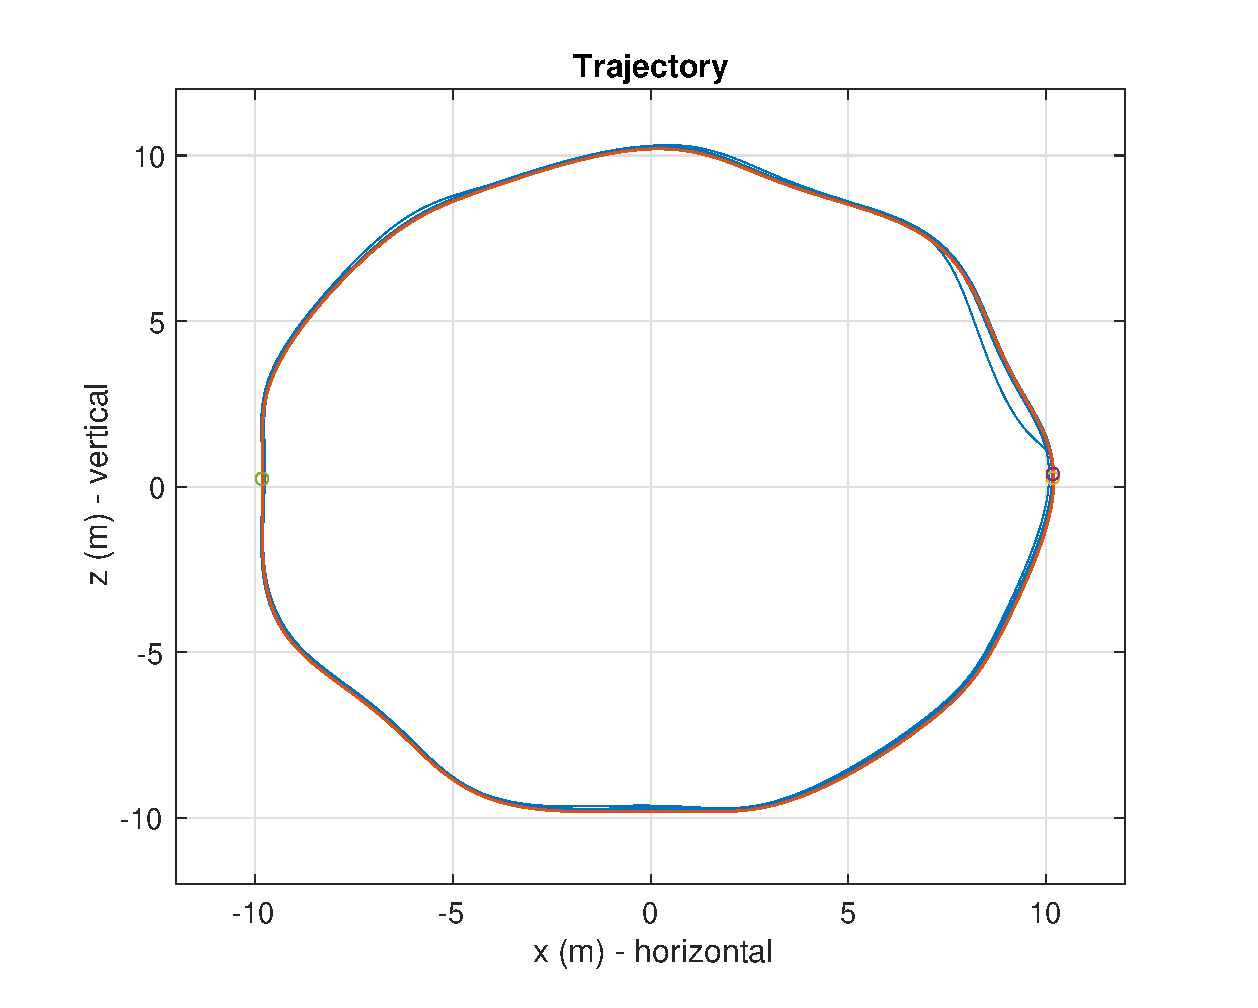
\includegraphics[width=0.4\textwidth]{circle_full_controller_traj}
	\caption{Tandem-rotor vehicle trajectory, with the full adaptive nonlinear sliding control architecture}
	\label{circle_traj_1}
\end{figure}

\begin{figure}[h!]
	\centering
	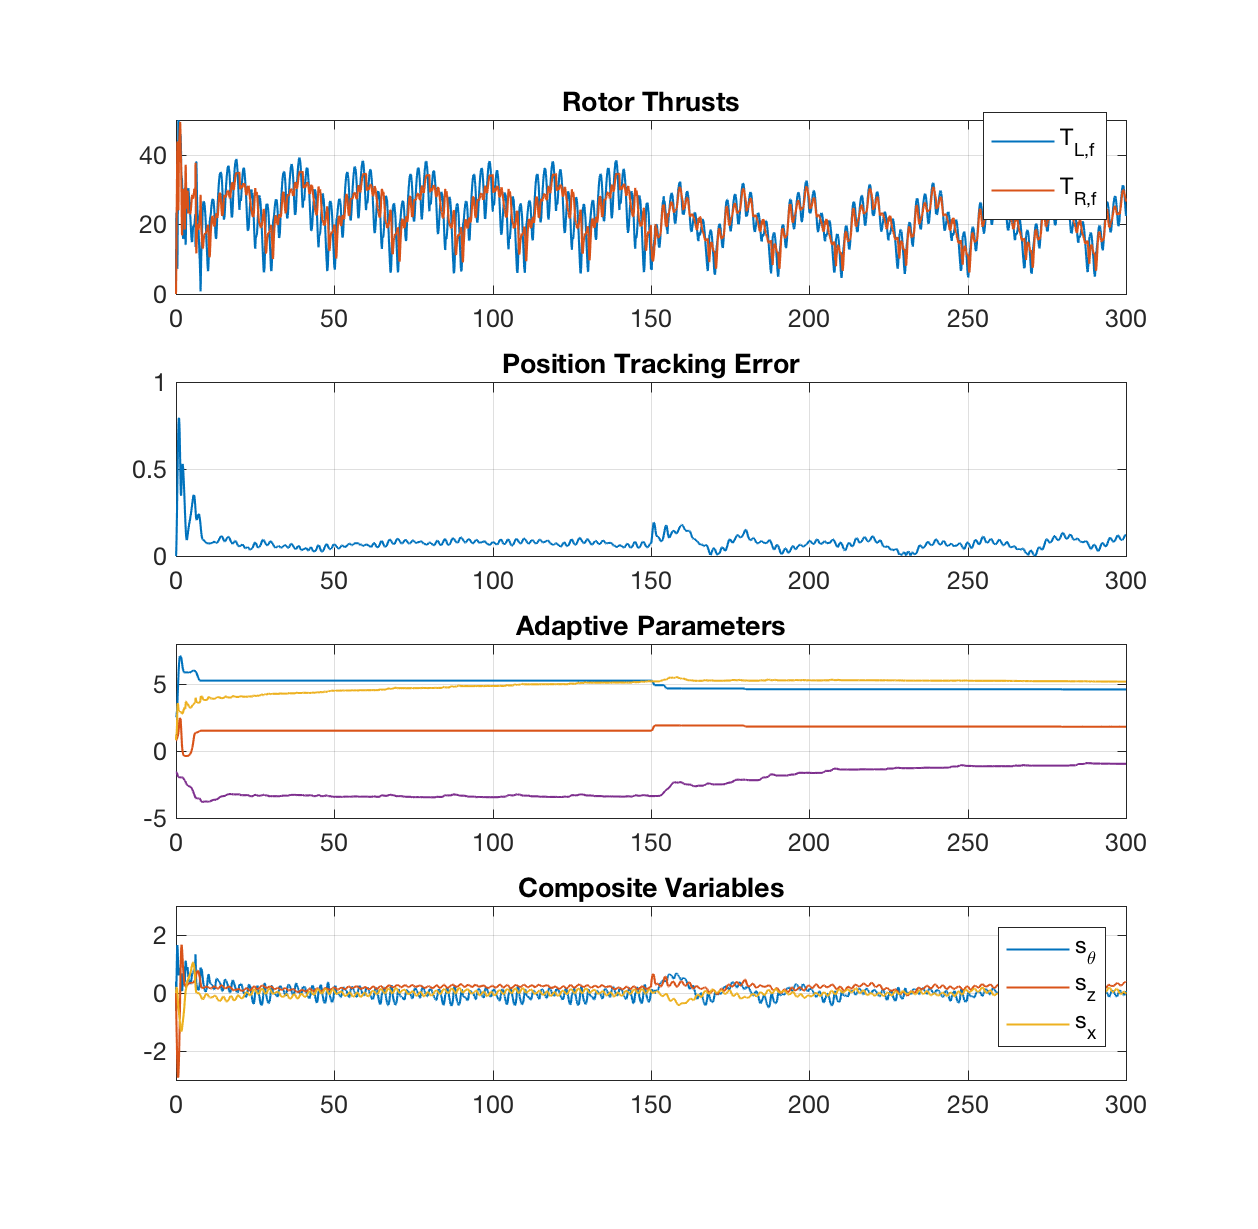
\includegraphics[width=0.5\textwidth]{circle_full_controller}
	\caption{Data associated with with trajectory in Fig. \ref{circle_traj_1}}
	\label{circle_data_1}
\end{figure}

\subsection{Nonlinear Controller - No Adaptation}
The test of this controller is shown in Figures \ref{circle_traj_2} and \ref{circle_data_2}. With this example, the adaptive parameters were all initialized to their correct values and adaptation was turned off ($\gamma_x = \gamma_z = \gamma_\theta = 0$). The desired trajectory is tracked until $t = 150s$, where the plant parameters change and the controller fails to adapt. A direct comparison with the example presented in this paper is shown in Figure \ref{traj_noadap}.

\begin{figure}[h!]
	\centering
	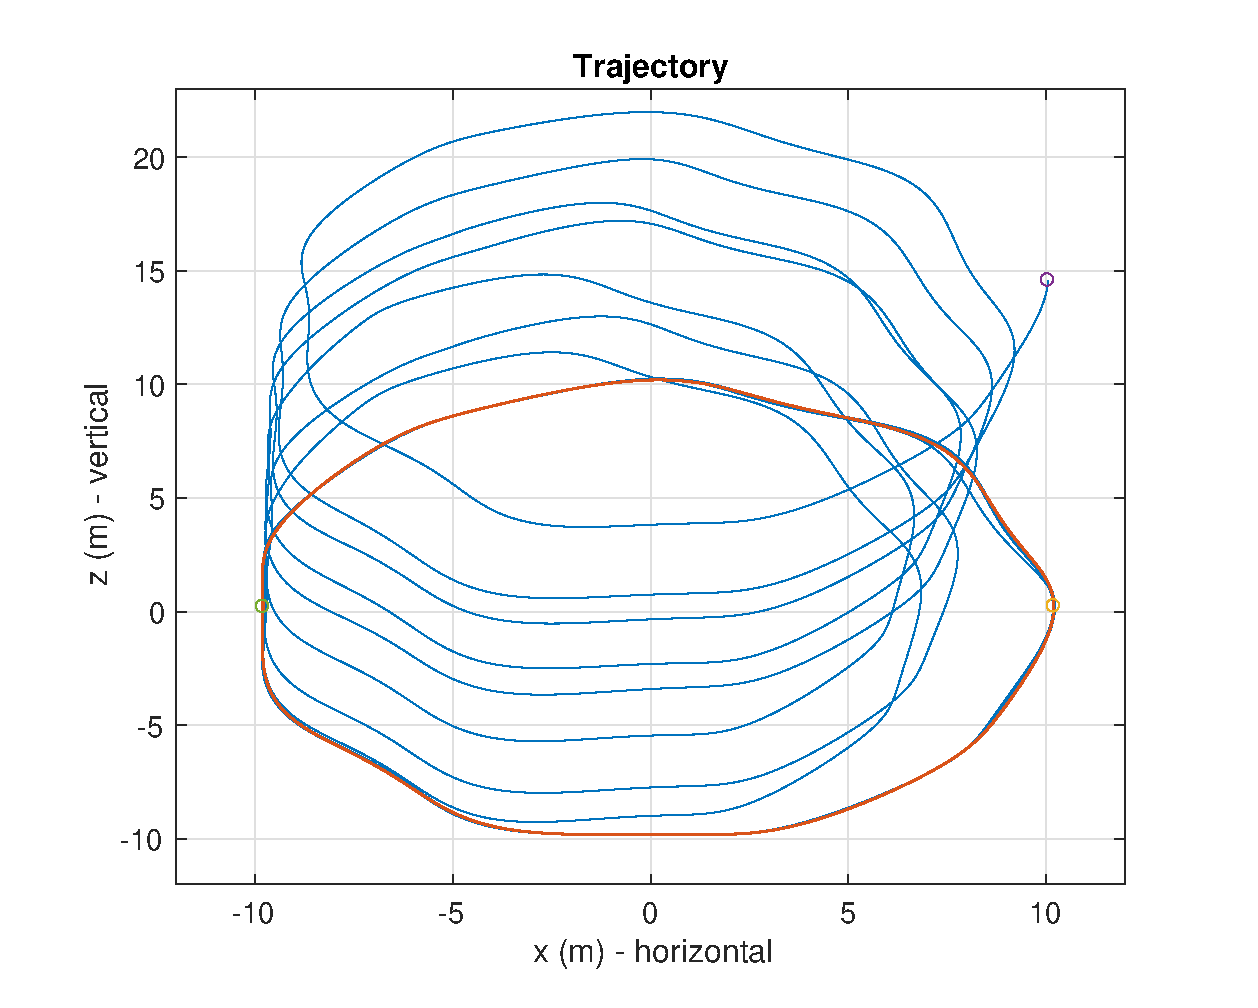
\includegraphics[width=0.4\textwidth]{circle_noadap_traj}
	\caption{Tandem-rotor vehicle trajectory, with the full nonlinear sliding control architecture but without adaptation}
	\label{circle_traj_2}
\end{figure}

\begin{figure}[h!]
	\centering
	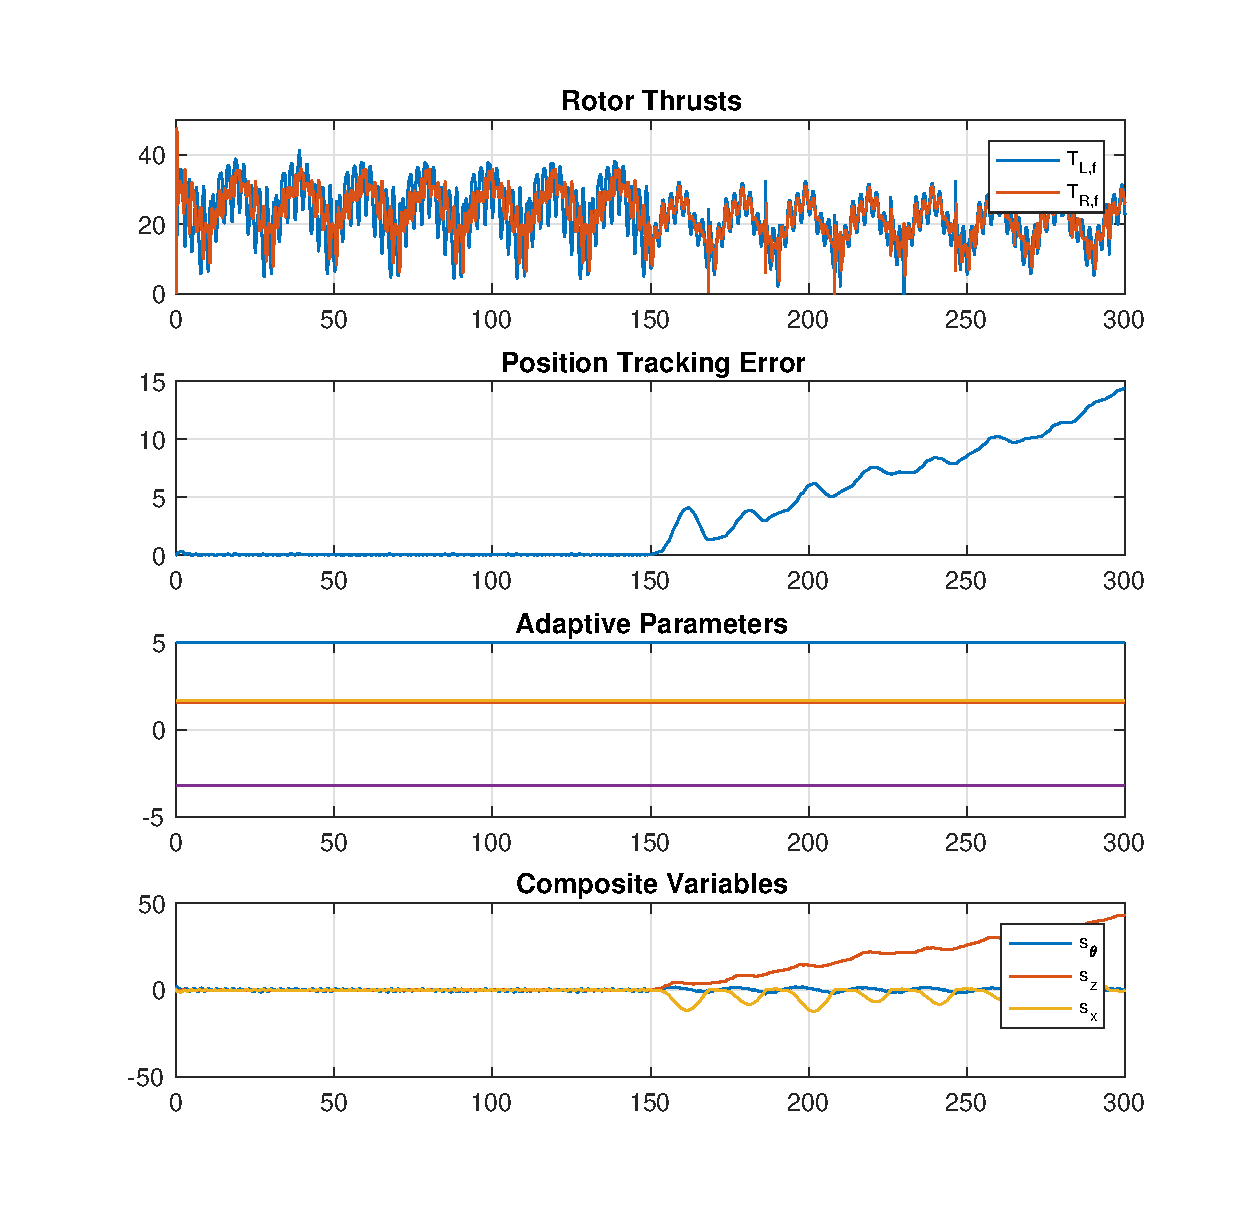
\includegraphics[width=0.5\textwidth]{circle_noadap}
	\caption{Data associated with with trajectory in Fig. \ref{circle_traj_2}}
	\label{circle_data_2}
\end{figure}

\begin{figure}
	\centering
	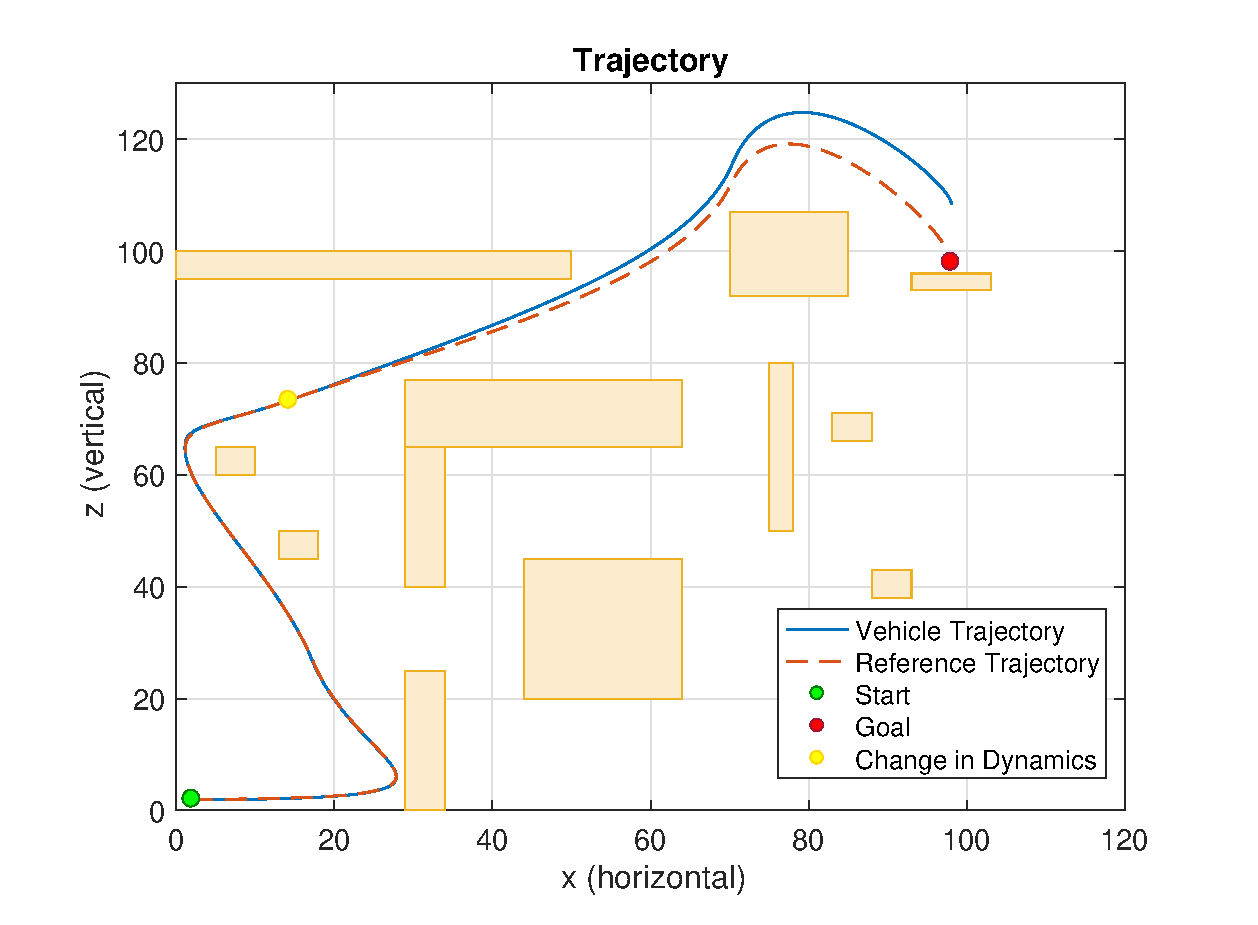
\includegraphics[width=0.5\textwidth]{traj_noadap}
	\caption{Tandem-rotor vehicle trajectory without adaptation, for comparison to Figure \ref{traj1}}
	\label{traj_noadap}
\end{figure}


\subsection{Linear Controller}
The test of this controller is shown in Figures \ref{circle_traj_3} and \ref{circle_data_3}. This controller uses the same parameters as that of Table \ref{plant_params_appendix}, but there is no feedforward action on the nonlinear damping ($\hat{a}_{out,2} = 0, \dot{\hat{a}}_{out,2} = 0$), and the nonlinear pitching moment from the unknown payload is linearized by approximating $\sin(\theta) = \theta$. Here, tracking performance is poor for the entire simulation.

\begin{figure}[h!]
	\centering
	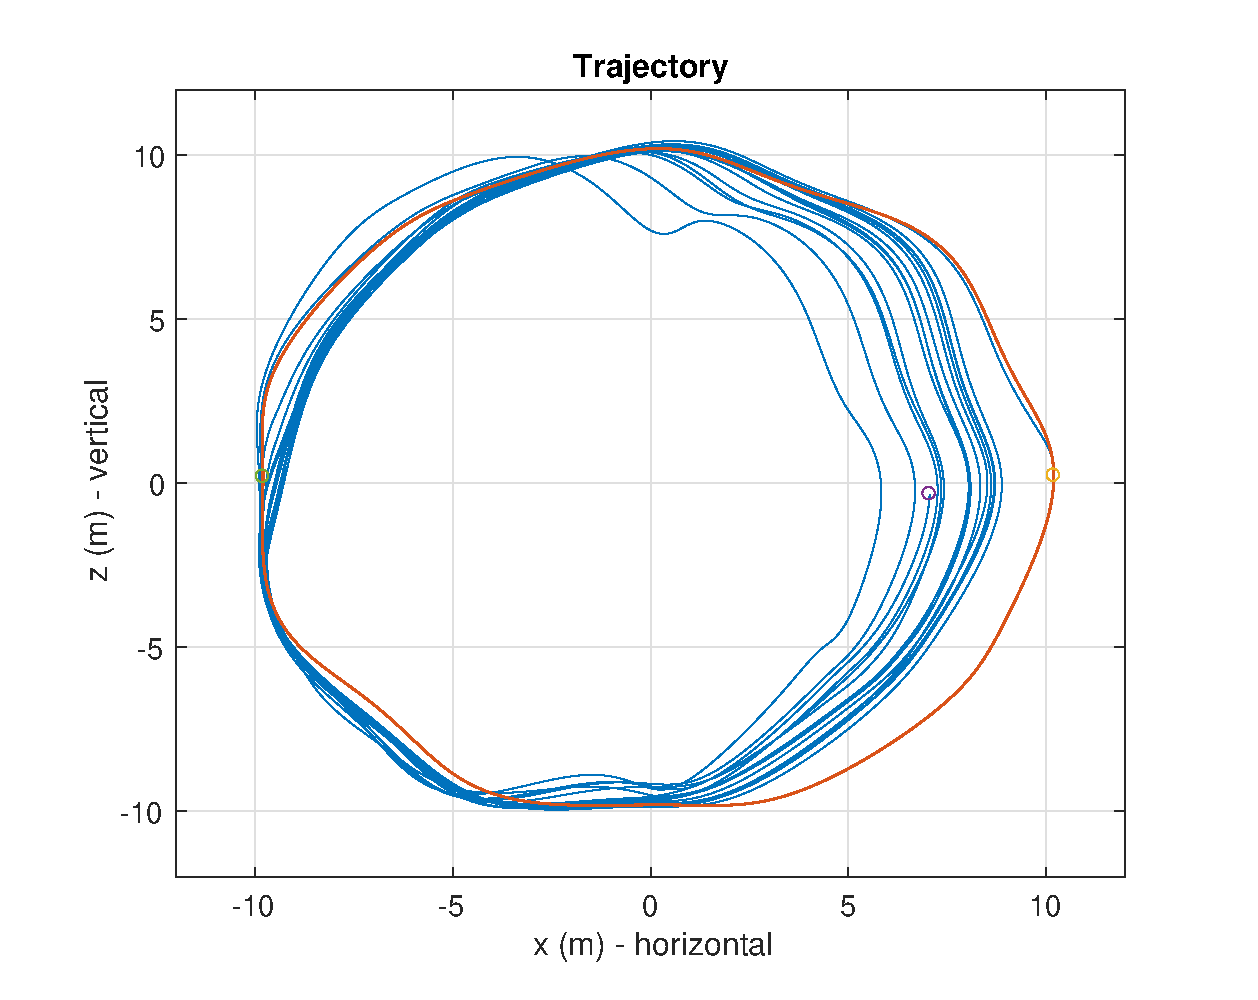
\includegraphics[width=0.4\textwidth]{circle_linear_traj}
	\caption{Tandem-rotor vehicle trajectory, with an adaptive sliding control architecture ignoring nonlinear damping and linearizing pitching moment near $\theta = 0$.}
	\label{circle_traj_3}
\end{figure}

\begin{figure}[h!]
	\centering
	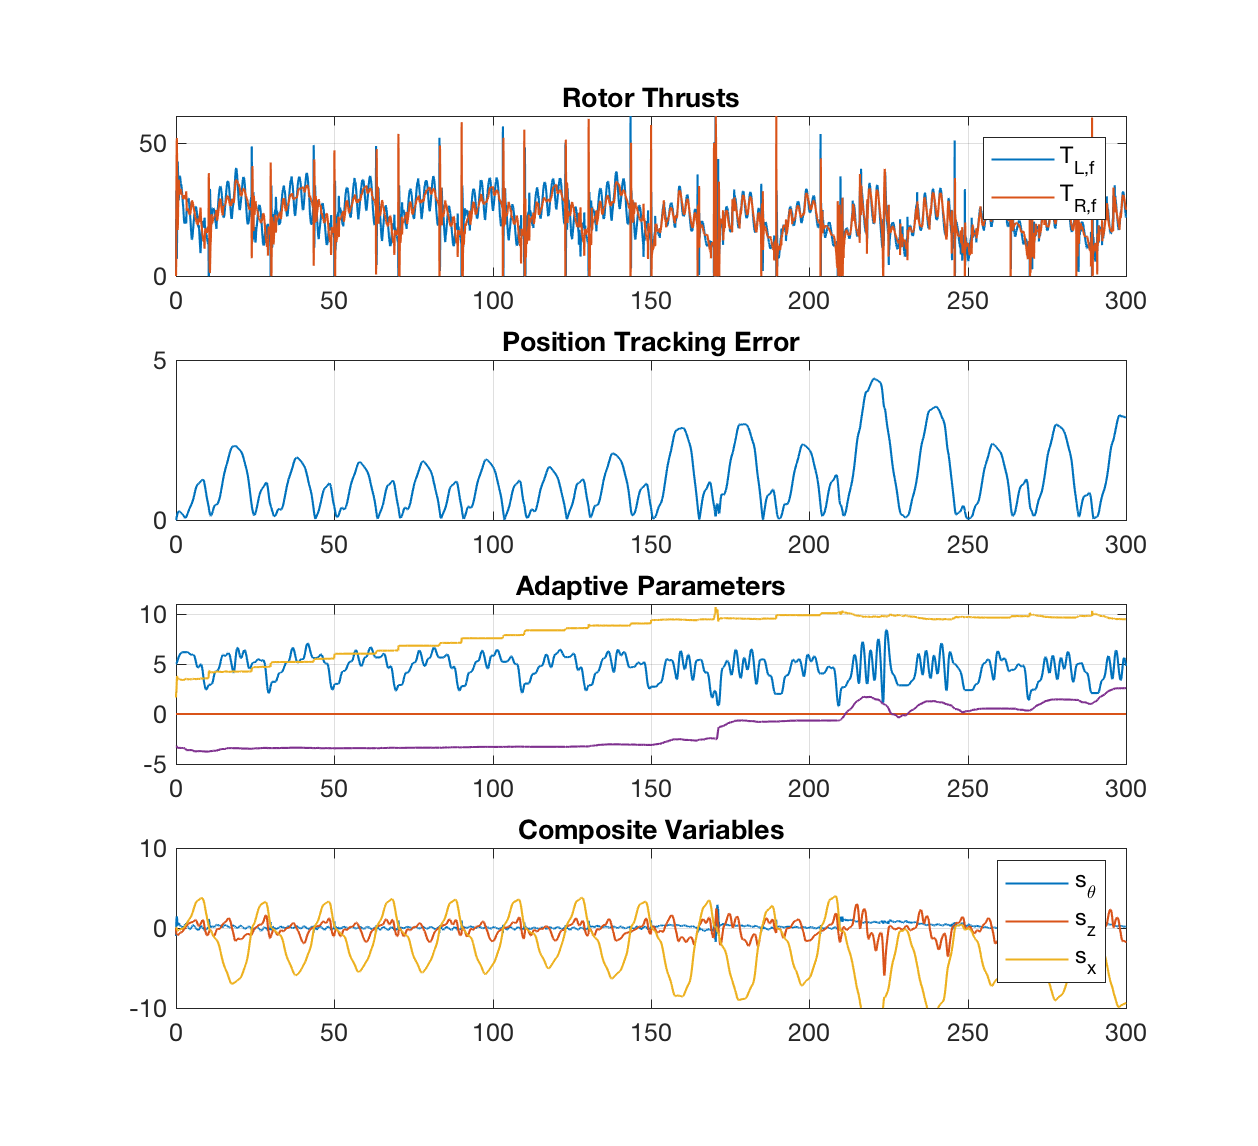
\includegraphics[width=0.5\textwidth]{circle_linear}
	\caption{Data associated with with trajectory in Fig. \ref{circle_traj_3}}
	\label{circle_data_3}
\end{figure}

\end{document}
